%main.tex
\documentclass[a4paper,11pt,twoside,ngerman,color]{book}
% header.tex

% Korrekte Darstellung der Umlaute (language and fonts)
\usepackage[T1]{fontenc} % T1-Fonts are better
\usepackage{lmodern} % Eine etwas angenehmere Font
\usepackage[utf8]{inputenc} % nutzt UTF8, bitte was sonst
\usepackage[main=ngerman]{babel} % Übersetze einige Literate auf Deutsch

% Math and theoretical computer science symboles/fonts
\usepackage{amsmath}  % American Math Society Packete: general
\usepackage{amsfonts} % American Math Society Packete: more fonts
\usepackage{amssymb}  % American Math Society Packete: more symbols
%\usepackage{amsthm}  % American Math Society Packete: typesetting theorems  %%% in conflict with ntheorem!!!
\usepackage{stmaryrd} % St Mary Road symbols for theoretical computer science
\usepackage{dsfont}   % supports the 1-function

% Caption Packet
\usepackage[margin=0pt,font=small,labelfont=bf]{caption} % cus­tomise the cap­tions in float­ing en­vi­ron­ments
% Gliederung einstellen
%\setcounter{secnumdepth}{5}
%\setcounter{tocdepth}{5}

% citations/ captions/ float­ing en­vi­ron­ments/ links
\usepackage{cite} % Improved Citation-Handling
\usepackage[babel,german=quotes,autostyle]{csquotes} % ad­vanced fa­cil­i­ties for in­line and dis­play quo­ta­tions
\MakeOuterQuote{"}	% for german style quotation marks
\usepackage{subcaption} % Support for sub-captions (and sub-figures)
\usepackage{enumerate} % Erweiterte Enumerate-Umgebungen
\usepackage{wrapfig} % Erlaubt es Text, Graphiken zu umfließen
\usepackage{lscape}
\usepackage{rotating}
%\usepackage{epstopdf}
\usepackage{float} % Verbesserte floating-objects
\usepackage{framed} % Umrahmte Abschnitte
\usepackage[framed,hyperref,amsmath,thmmarks]{ntheorem} % en­hance­ments for the­o­rem-like en­vi­ron­ments
\usepackage[unicode,pdfmenubar,linktoc=all,hidelinks,bookmarks]{hyperref} % ermöglicht PDF-Verklinkungen
\usepackage{url} % al­lows line­breaks at cer­tain char­ac­ters in urls/ e-mail adresses/ paths
\usepackage{multicol} % to use columns with multiple rows

% Abkuerzungen richtig formatieren %
\usepackage{xspace}

% Euro Symbol
\usepackage{eurosym}

% Seitenlayout
\usepackage{geometry} % Beinflusst das Seitenlayout
\geometry{a4paper} % Papiergroesse
%%\geometry{top=25mm, inner=25mm, outer=25mm, bottom=25mm, headsep=10mm, footskip=10mm} % Seitenraender
%%\geometry{left=3.5cm,right=2.5cm,bottom=3.5cm,top=3cm} % Seitenraender
\usepackage{pdflscape} % Landscape Umgebung für PDF Dokumente: set­ting the page at­tribute /Ro­tate 
\usepackage[hang]{footmisc}   % Für den Einzug bei Fußnoten
\setlength{\footnotemargin}{0pt} % Setze den Einzug für die Fußnoten
\parskip 0pt
%\parindent 0pt

% Grafiken
\usepackage[pdftex]{color} % Erweiterter Support für Graphiken
\usepackage{graphicx}
%\usepackage{subfigure}
\usepackage{tikz} % Für LaTeX Graphiken
\usetikzlibrary{automata,arrows,backgrounds,decorations.markings,decorations.pathmorphing,decorations.pathreplacing,fit,positioning,shadows,shapes,shapes.geometric} % Ein paar nützliche TikZ-Pakete


% Bibtex deutsch
\usepackage{bibgerm}

\usepackage{makeidx} % Index für Schlagwörter
\makeindex

\usepackage[final]{listofsymbols}  % Symbolverzeichnis
%\usepackage[draft]{listofsymbols}


% Zeilenabstand einstellen %
\renewcommand{\baselinestretch}{1.25}
% Floating-Umgebungen anpassen %
\renewcommand{\topfraction}{0.9}
\renewcommand{\bottomfraction}{0.8}

% Keine einzelnen Zeilen beim Anfang eines Abschnitts (Schusterjungen)
\clubpenalty = 10000
% Keine einzelnen Zeilen am Ende eines Abschnitts (Hurenkinder)
\widowpenalty = 10000 \displaywidowpenalty = 10000
% EOF

 % Seitenraender %
\geometry{left=3.5cm,right=2.5cm,bottom=3.5cm,top=3cm}

% Algorithmen
\usepackage[plain,chapter]{algorithm}
\usepackage{algorithmic}
%\usepackage{algpseudocode}

% Tabellen
%\usepackage{booktabs}  % Statt \hline kann \toprule, \midrule und \bottomrule verwendet werden.
%\usepackage{multirow} % provides a construction for table cells that span more than one row
%\usepackage{multicol} % allows switching between one and multicolumn format on the same page

% theoremOptions.tex

% Theorem-Optionen %
\theoremseparator{.}
\theoremstyle{change}
\newtheorem{theorem}{Theorem}[section]
\newtheorem{satz}[theorem]{Satz}
\newtheorem{lemma}[theorem]{Lemma}
\newtheorem{korollar}[theorem]{Korollar}
\newtheorem{proposition}[theorem]{Proposition}
% Ohne Numerierung
\theoremstyle{nonumberplain}
\renewtheorem{theorem*}{Theorem}
\renewtheorem{satz*}{Satz}
\renewtheorem{lemma*}{Lemma}
\renewtheorem{korollar*}{Korollar}
\renewtheorem{proposition*}{Proposition}
% Definitionen mit \upshape
\theorembodyfont{\upshape}
\theoremstyle{change}
\newtheorem{definition}[theorem]{Definition}
\theoremstyle{nonumberplain}
\renewtheorem{definition*}{Definition}
% Kursive Schrift
\theoremheaderfont{\itshape}
\newtheorem{notation}{Notation}
\newtheorem{konvention}{Konvention}
\newtheorem{bezeichnung}{Bezeichnung}
\theoremsymbol{\ensuremath{\Box}}
\newtheorem{beweis}{Beweis}
\theoremsymbol{}
\theoremstyle{change}
\theoremheaderfont{\bfseries}
\newtheorem{bemerkung}[theorem]{Bemerkung}
\newtheorem{beobachtung}[theorem]{Beobachtung}
\newtheorem{beispiel}[theorem]{Beispiel}
\newtheorem{problem}{Problem}
\theoremstyle{nonumberplain}
\renewtheorem{bemerkung*}{Bemerkung}
\renewtheorem{beispiel*}{Beispiel}
\renewtheorem{problem*}{Problem}
%EOF
% algorithmOptions.tex

% Algorithmen anpassen %
\renewcommand{\algorithmicrequire}{\textbf{Eingabe:}\@\xspace}
\renewcommand{\algorithmicensure}{\textbf{Ausgabe:}\@\xspace}
\floatname{algorithm}{Algorithmus}
\renewcommand{\listalgorithmname}{Algorithmenverzeichnis}
\renewcommand{\algorithmiccomment}[1]{\hfill\color{gray}{// #1}\color{black}}
%EOF
%% pseudoCodeOptions.tex

% pseudocode Einstellungen
\usepackage{listings} % for type­set pro­gram­ming code
\lstset{
  language=Java,
  basicstyle=\ttfamily,
  commentstyle=\color{darkgreen},
  keywordstyle=\bfseries\color{darkblue},
  stringstyle=\color{darkred},
  showspaces=false,
  showstringspaces=false,
  showtabs=false,
  columns=fixed,
  frame=single,
  numbers=left,
  numberstyle=\tiny,
  numbersep=5pt,
  breaklines=true,
  backgroundcolor=\color{lightblue},
  captionpos=b
}
% Python style for highlighting
\newcommand\pythonstyle{\lstset{
language=Python,
basicstyle=\ttm,
otherkeywords={self},             % Add keywords here
keywordstyle=\ttb\color{deepblue},
emph={MyClass,__init__},          % Custom highlighting
emphstyle=\ttb\color{deepred},    % Custom highlighting style
stringstyle=\color{deepgreen},
frame=tb,                         % Any extra options here
showstringspaces=false            % 
}}
%EOF
% customCommands.tex
\usepackage{xparse}


% shortcuts for mathstuff
\newcommand{\Bed}{\mid}
\newcommand{\Oder}{\ \vee \ }
\newcommand{\Und}{\ \wedge \ }
\newcommand{\argmax}{\text{argmax}}
\newcommand{\GDW}{\Leftrightarrow}
\newcommand{\gdw}{genau dann, wenn\@\xspace}

% Abkuerzungen richtig formatieren %
\newcommand{\vgl}{vgl.\@\xspace} 
\newcommand{\zB}{z.\nolinebreak[4]\hspace{0.125em}\nolinebreak[4]B.\@\xspace}
\newcommand{\bzw}{bzw.\@\xspace}
\newcommand{\dahe}{d.\nolinebreak[4]\hspace{0.125em}h.\nolinebreak[4]\@\xspace}
\newcommand{\etc}{etc.\@\xspace}
\newcommand{\evtl}{evtl.\@\xspace}
\newcommand{\insb}{insb.\@\xspace}
\newcommand{\ggf}{ggf.\@\xspace}
\newcommand{\bzgl}{bzgl.\@\xspace}
\newcommand{\so}{s.\nolinebreak[4]\hspace{0.125em}\nolinebreak[4]o.\@\xspace}
\newcommand{\iA}{i.\nolinebreak[4]\hspace{0.125em}\nolinebreak[4]A.\@\xspace}
\newcommand{\sa}{s.\nolinebreak[4]\hspace{0.125em}\nolinebreak[4]a.\@\xspace}
\newcommand{\sAbb}{s.\nolinebreak[4]\hspace{0.125em}\nolinebreak[4]Abb.\@\xspace}
\newcommand{\sS}{s.\nolinebreak[4]\hspace{0.125em}\nolinebreak[4]S.\@\xspace}
\newcommand{\su}{s.\nolinebreak[4]\hspace{0.125em}\nolinebreak[4]u.\@\xspace}
\newcommand{\ua}{u.\nolinebreak[4]\hspace{0.125em}\nolinebreak[4]a.\@\xspace}
\newcommand{\og}{o.\nolinebreak[4]\hspace{0.125em}\nolinebreak[4]g.\@\xspace}
\newcommand{\oBdA}{o.\nolinebreak[4]\hspace{0.125em}\nolinebreak[4]B.\nolinebreak[4]\hspace{0.125em}d.\nolinebreak[4]\hspace{0.125em}A.\@\xspace}
\newcommand{\OBdA}{O.\nolinebreak[4]\hspace{0.125em}\nolinebreak[4]B.\nolinebreak[4]\hspace{0.125em}d.\nolinebreak[4]\hspace{0.125em}A.\@\xspace}
\newcommand{\engl}{engl.\@\xspace}
\newcommand{\Abb}{Abb.\@\xspace}

% Leere Seite ohne Seitennummer, naechste Seite rechts
\newcommand{\blankpage}{
 \clearpage{\pagestyle{empty}\cleardoublepage}
}
%EOF
%symbols.tex
\opensymdef
\newsym[Menge aller nat"urlichen Zahlen ohne die Null]{symnz}{\mathds{N}}
\newsym[Menge aller nat"urlichen Zahlen einschlie"slich Null]{symnzmn}{\mathds{N}_{0}}
\newsym[Menge aller ganzen Zahlen]{GZ}{\mathds{Z}}
\newsym[Menge aller rationalen Zahlen]{RatZ}{\mathds{Q}}
\newsym[Menge aller reellen Zahlen]{RZ}{\mathds{R}}
\newsym[euklidische Ebene]{RE}{\mathds{R}^2}
\newsym[Graph]{Graph}{G}

\closesymdef


% % % % % % % % % % % % % % % % % % % % % % % % % % % % % % % % % % % % % % % % % % % % % % %
% HIER eigene Angaben ERGÄNZEN:
% % % % % % % % % % % % % % % % % % % % % % % % % % % % % % % % % % % % % % % % % % % % % % %
% title.tex

\newcommand{\MeinVorame}{Julian\@\xspace}
\newcommand{\MeinNachname}{Sauer\@\xspace}
\newcommand{\MeineMatrikelnummer}{197859\@\xspace}

\newcommand{\MeineArbeit}{Masterarbeit\@\xspace}
%\newcommand{\MeineArbeit}{Masterarbeit\@\xspace}

\newcommand{\MeinTitel}{Effiziente Berechnung von $K_5$-Minoren in Graphen}

%\newcommand{\Erstbetreuer}{Name des Erstbetreuers}
\newcommand{\Erstbetreuer}{Prof.\ Dr.\ Petra Mutzel}
%\newcommand{\Erstbetreuer}{Prof.\ Dr.\ Sven Rahmann}
%\newcommand{\Erstbetreuer}{Prof.\ Dr.\ Günter Rudolph}
%\newcommand{\Erstbetreuer}{Prof.\ Dr.\ Johannes Fischer}
\newcommand{\Zweitbetreuer}{Prof.\ Dr.\ Jens Schmidt}
%EOF

% % % % % % % % % % % % % % % % % % % % % % % % % % % % % % % % % % % % % % % % % % % % % % %

\begin{document}
% Titelseite
\begin{titlepage}
\vspace*{-2cm}
\newlength{\links}
\setlength{\links}{-1.5cm}
\sf
\LARGE

\hspace*{\links}
\begin{minipage}{12.5cm}

\includegraphics[width=8cm]{bilder/tulogo-rgb}
%\hspace*{-0.25cm} \textbf{TECHNISCHE UNIVERSITÄT DORTMUND}\\
%\hspace*{-1.2cm} \rule{5mm}{5mm} \hspace*{0.1cm} FACHBEREICH INFORMATIK\\
\end{minipage}

\vspace*{4cm}

\hspace*{\links}
\hspace*{-0.2cm}
\begin{minipage}{8.5cm}
\large
\begin{center}
{\Large \MeineArbeit} \\
\vspace*{1cm}
\bf{ \MeinTitel } \\
\vspace*{1.5cm}
\MeinVorame \MeinNachname\\
\today
\end{center}
\end{minipage}

\vspace*{3.7cm}

\hspace*{\links}

\vspace*{1.5cm}

\vspace*{.6cm}

\hspace*{\links}
\begin{minipage}[b]{5cm}
\normalsize
\raggedright
Betreuer: \\
\Erstbetreuer \\
\Zweitbetreuer \\
\end{minipage}

\definecolor{TUGreen}{rgb}{0.517,0.721,0.094}
\vspace*{2.5cm}
\hspace*{\links}
\begin{minipage}[b]{8cm}
\normalsize
\raggedright
Fakultät für Informatik\\
Algorithm Engineering (LS 11)\\
Technische Universität Dortmund \\
http://ls11-www.cs.tu-dortmund.de
\end{minipage}


\end{titlepage}

\blankpage
%\include{chapters/titelseite_innen}
%\blankpage

\pagenumbering{roman}
\tableofcontents
\cleardoublepage
\pagenumbering{arabic}

% Kapitel
% einleitung.tex
\chapter{Einleitung}
\label{cha:einleitung}

Im Rahmen dieser Masterarbeit wird ein Algorithmus erklärt und implementiert, der entscheiden kann, ob ein Graph \kf-Minor-frei ist.
Er basiert auf einem von Kezdy und McGuinness \cite{KeM92} vorgestellten Algorithmus, der quadratische Laufzeitkomplexität besitzt.

\section{Motivation und Hintergrund}
\label{sec:motivation_und_hintergrund}
Durch die Berechnung von \kf-Minoren kann entschieden werden, ob ein Graph \kf-Minor-frei ist.
Das ist insofern interessant, als dass einige Algorithmen effizienter auf \kf-Minor-freien Graphen ausgeführt werden können.
So ist die Berechnung eines \emph{maximalen Schnittes} (\emph{Max-Cut Problem}) - also das Aufteilen der Knoten eines Graphen in zwei Mengen, sodass die Kanten zwischen diesen beiden Mengen in Summe ein maximales Gewicht besitzen - NP-schwer\cite{Kar72}.
Allerdings wird etwa in \cite{Bar83} gezeigt, dass es für Graphen ohne \kf-Minor in Polynomialzeit gelöst werden kann.
Viele kombinatorische Optimierungsprobleme wie quadratische 0-1 Probleme können als Max-Cut Probleme formuliert werden\cite{BJR89}, sodass \kf-Minor-freie Probleminstanzen deutlich effizienter gelöst werden können.

In \cite{JLMR+19} transformieren Jünger et al.\nolinebreak[4]\@\xspace Ising Spin Glass Probleme zu Max-Cut Problemen, um mit Hilfe von einem Branch-and-Cut Algorithmus eine optimale Lösung zu finden.
Diese kann mit den heuristischen Lösungen, die etwa auf dem Quantencomputer \emph{D-Wave 2000Q} berechnet werden, verglichen werden.
Dadurch kann beispielsweise bewertet werden, ob für die schnellere Laufzeit des Quantencomputers die heuristische Lösung tragbar ist.
Innerhalb des exakten Verfahrens stellen die \kf-Minoren die Schwierigkeit des Problems dar.
Deshalb kann das Problem einerseits für \kf-Minor-freie Graphen effizient gelöst werden.
Andererseits können einer oder mehrere gefundene \kf-Minoren benutzt werden, um innerhalb des linearen Programms den Suchraum zu beschränken und die Berechnung zu beschleunigen.

\section{Aufbau der Arbeit}
\label{sec:aufbau}
Zunächst werden einige Definition gegeben, die anschließend benutzt werden, um den Algorithmus von Kezdy und McGuinness \cite{KeM92} vorzustellen.
Anschließend wird ein auf Wagner \cite{Wag37} zurückzuführendes Strukturtheorem der beiden Autoren genauer betrachtet.
Für den Fall, dass ein Graph \kf-Minor-frei ist, kann dadurch ein Zertifikat erzeugt werden, über dass die getroffene Aussage verifiziert werden kann.
Letztlich beschäftigt sich die Arbeit mit der Implementierung des Algorithmus im \emph{Open Graph Drawing Framework} sowie einer experimentellen Analyse dieser Implementierung.

% kapitel2.tex
\chapter{Definitionen}
\label{cha:definitionen}

Vorab werden einige Definitionen und Notationen festgelegt, die im Verlauf der Arbeit verwendet werden.
Der Algorithmus arbeitet mit einem ungerichteten Graph $G = (V, E)$ ohne Mehrfachkanten, wobei $E$ die Menge der Kanten und $V$ die Knotenmenge sei.
\begin{wrapfigure}{r}{6cm}
  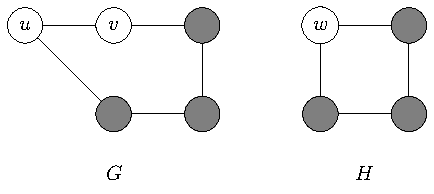
\includegraphics[width=6cm]{bilder/Kantenkontraktion.pdf}
  \caption{Die Kante, die $u$ und $v$ in $G$ verbindet, wird kontrahiert, sodass sie in $H$ durch den neuen Knoten $w$ ersetzt wird.}
  \label{fig:Kantenkontraktion}
\end{wrapfigure}
Eine Kante $e \in E$, die zwei Knoten $u$ und $v$ verbindet, wird durch $e = (u, v)$ angegeben.
Ein Pfad $P(u, v)$ verbindet zwei Knoten $u$ und $v$ über eine Folge von Knoten, die adjazent zueinander sind.
Bei der Kontraktion einer Kante $e = (u, v)$ wird diese mit ihren beiden Endpunkten aus dem Graph entfernt und einen neuen Knoten $w$ ersetzt.
Die Nachbarknoten von $w$ werden auf die Menge der adjazenten Knoten von $u$ und $v$ gesetzt.
In Abbildung \ref{fig:Kantenkontraktion} ist das Vorgehen skizziert.
Analog kann, wie in Abbildung \ref{fig:Pfadkontraktion} gezeigt, ein Pfad kontrahiert werden, wobei der neu eingefügte Knoten $w$ Kanten zu der Menge der adjazenten Knoten aller Knoten des Pfades besitzt.
\begin{wrapfigure}{l}{6cm}
  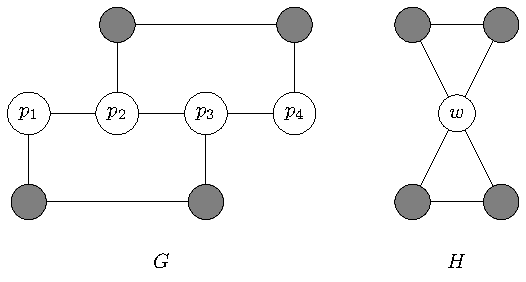
\includegraphics[width=6cm]{bilder/Pfadkontraktion.pdf}
  \caption{Der Pfad von $p_1$ bis $p_4$ wird kontrahiert.
           Der neue Knoten $w$ in $H$ enthält alle Nachbarn der Pfadknoten in $G$.}
  \label{fig:Pfadkontraktion}
\end{wrapfigure}

Ein Minor $H$ eines Graphen $G$ bezeichnet einen Graph, der isomorph zu $G$ ist, nachdem eine beliebige Menge an Operationen von Kantenkontraktionen, Kantenentfernungen und Knotenentfernungen durchgeführt wurde.
Ein Beispiel dazu findet sich in Abbildung \ref{fig:Minor}.
Jeder Graph ist sein eigener Minor, genauso ist jeder Teilgraph ein gültiger Minor.
Dass $H$ ein Minor von $G$ ist, wird dargestellt durch $H$ \minor $G$.
Das Branch-Set eines Knotens $w$ aus einem Minor von $G$ bezeichnet die Menge an Knoten, die durch Kontraktionen zu $w$ verschmolzen wurden.
In Abbildung \ref{fig:Minor} besteht beispielsweise das Branch-Set von $g$ aus $\{a, b, c\}$, zu $f$ in $H_2$ gehört die Knotenmenge $\{f\}$ in $G$.
Für die Knotenmenge $U \in V$ bezeichnet $G \setminus U$ den Teilgraph, der entsteht, wenn alle Knoten aus $U$ mit ihren inzidenten Kanten aus $G$ entfernt werden.
Ein Homöomorph eines Graphen $G$ enthält alle Knoten und Kanten aus $G$, zusätzlich können aber Kanten als gegenteilige Operation zur Kontraktion unterteilt werden.
Für eine Kante $e = (u, v)$ bedeute das, dass $e$ entfernt wird, dafür ein neuer Knoten $w$ und zwei neue Kanten $(u, w)$ und $(w, v)$ eingefügt werden.
\begin{figure}[H]
  \centering
  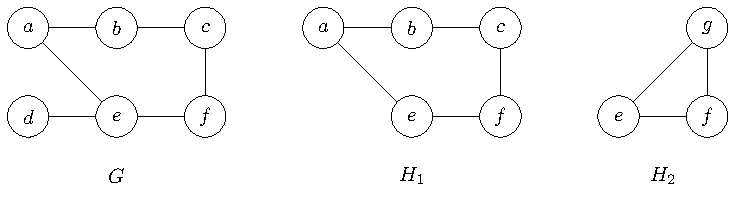
\includegraphics[keepaspectratio]{bilder/Minor.pdf}
  \caption{Ein Graph $G$ mit seinen Minoren $H_1$ und $H_2$.
           Um $H_1$ zu erhalten, wurde in $G$ die Kante $(d, e)$ und anschließend der Knoten $d$ entfernt.
           Für $H_2$ wurden außerdem der Pfad $P(a, c)$ kontrahiert.}
  \label{fig:Minor}
\end{figure}

\begin{wrapfigure}{r}{4cm}
  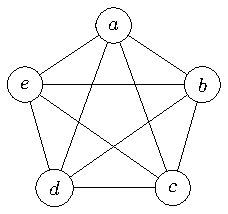
\includegraphics[width=4cm]{bilder/K_5.pdf}
  \caption{Der Graph \kf.}
  \label{fig:K5}
\end{wrapfigure}
Ein Graph wird als planar bezeichnet, wenn er sich so in der Ebene einbetten lässt, dass sich keine Kanten kreuzen.
Ein \kf (\sAbb \ref{fig:K5}) ist ein spezieller Graph, der aus fünf Knoten besteht, die alle zueinander adjazent sind.
Ein \kdd (\sAbb \ref{fig:K33}) ist ein vollständig bipartiter Graph mit sechs Knoten.
Er lässt sich also in zwei Knotenmengen unterteilen (im Folgenden als rote und blaue Menge bezeichnet), sodass alle Knoten der einen Menge zu allen Knoten der anderen Menge benachbart sind.
Nach dem Satz von Kuratowski ist ein Graph planar, wenn er kein \kf- oder \kdd-Homöomorph als Teilgraph beinhaltet.
Eine alternative Formulierung von Wagner sagt aus, dass ein Graph planar ist, wenn er keinen \kf-Minor oder \kdd-Minor enthält.\cite{Die12}
\begin{wrapfigure}{r}{4cm}
  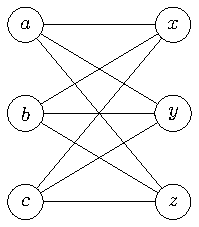
\includegraphics[width=4cm]{bilder/K_33.pdf}
  \caption{Der Graph \kdd.}
  \label{fig:K33}
\end{wrapfigure}

Als nächstes wird ein \kdd genauer betrachtet.
Sei dessen rote Knotenmenge $R = \{a, b, c\}$ und blaue $B = \{x, y, z\}$
Diese sechs Knoten werden in einem \kdd-Homöomorph $H$ als Branch-Ends genannt und zeichnen sich dadurch aus, dass sie als einzige Knoten in $H$ den Grad 3 haben.
Ein Branch-Path in $H$ ist ein Pfad, der zwei Branch-Ends verbindet, beispielsweise $P(a, x)$.
Ein Branch-Fan bezieht sich immer auf einen der Branch-Ends und wird \zB für $a$ als $F(a)$ geschrieben.
Bezeichnet werden dadurch alle Pfade, die zu einem anderen Branch-End führen - für $a$ also die Pfade $P(a, x)$, $P(a, y)$ und $P(a, z)$.


Der Graph $W$ bezeichnet einen speziellen Graph, der aus acht Knoten besteht.
Seine äußeren Kanten bilden einen Kreis, außerdem sind die Knoten jeweils adjazent zu den gegenüberliegenden. Eine Darstellung findet sich links in Abbildung \ref{fig:W}.
Er enthält einen \kdd als Minor (in der Abbildung rechts angedeutet), jedoch keinen \kf.
Als $M$ wird ein Graph bezeichnet, der einen \kdd als Teilgraph enthält, jedoch einen zusätzlichen Knoten und zwei zusätzliche Kanten enthält.
Er ist insofern interessant, als dass er, wie in Abbildung \ref{fig:M} zu sehen, neben einem \kdd-Minor auch einen \kf-Minor enthält.
\begin{figure}[H]
  \centering
  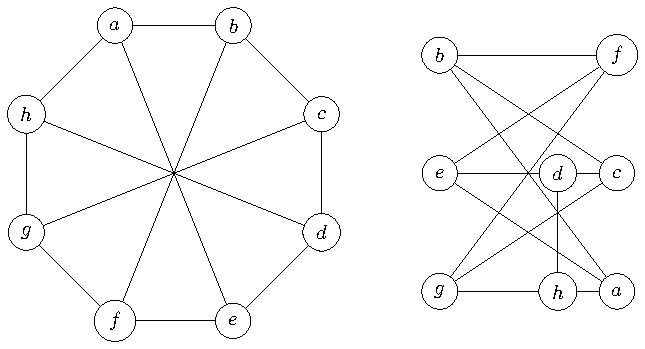
\includegraphics[keepaspectratio]{bilder/W.pdf}
  \caption{Der Graph $W$, links in seiner üblichen Darstellung, rechts mit angedeutetem \kdd-Minor.}
  \label{fig:W}
\end{figure}

\begin{figure}[H]
  \centering
  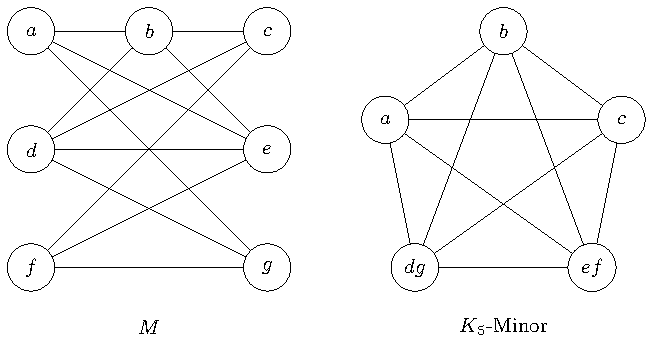
\includegraphics[keepaspectratio]{bilder/M.pdf}
  \caption{Der Graph $M$ sowie ein \kf-Minor aus $M$.}
  \label{fig:W}
\end{figure}

Als $(i)$-Separator wird eine Menge $S$ bestehend aus $i$ Knoten in einem zusammenhängenden Graph $G$ bezeichnet, sodass $G \setminus S$ nicht mehr zusammenhängend ist.
Ein $(i, j)$-Separator ist ein $i$-Separator, sodass $G-S$ aus mindestens $j$ Zusammenhangskomponenten besteht.
In Abbildung \ref{fig:AugmentierteKomponenten} wird ein \dd-Separator im linken Graph gezeigt.
Durch einen Separator können augmentierte Komponenten definiert werden:
Sind $C \in V$ die $i$ Knoten, die zu einem $(i, j)$-Separator in $G$ gehören, wird der Graph durch $G \setminus C$ zunächst in $j$ Zusammenhangskomponenten zerlegt.
Anschließend werden Kopien der Knoten aus $C$ zu jeder Komponente hinzugefügt.
Sie bilden dabei in jeder Zusammenhangskomponente eine Clique.
Außerdem besitzen sie Kanten zu Knoten in der Zusammenhangskomponente, falls eine Kante $e = (c, z)$ in $G$ existierte, $c \in C$ und $z$ ein Knoten der Zusammenhangskomponente ist.
Jeder der resultierenden Graphen ist eine augmentierte Komponente des Urpsrungsgraphen $G$ und wie in Theorem \ref{Theorem33} bewiesen wird, \evtl ein Minor zu $G$.
Als gegenteilige Operation kann eine Cliquen-Summe verwendet werden, um zwei Graphen zu verschmelzen.
Dazu müssen zwei Graphen $H_1$ und $H_2$ als Teilgraph eine gleich große Clique enthalten.
$H_1$ und $H_2$ können zu einem Graph zusammengefügt werden, indem je ein Knoten von der Clique in $H_1$ und in $H_2$ zu einem zusammengefügt werden.
Im resultiernden Graph dürfen außerdem Kanten zwischen den Knoten der Clique entfernt werden.
Dadurch ist es möglich, einen Graph $G$ in augmentierte Komponente zu zerlegen und anschließend durch eine Cliquen-Summe wieder $G$ zu erhalten.
Dieses Vorgehen wird in Abbildung \ref{fig:AugmentierteKomponenten} gezeigt, dabei wird der linke Graph rechts in augmentierte Komponenten zerlegt \bzw von rechts nach links werden drei Graphen durch eine Cliquen-Summe zusammengefügt.
\begin{figure}[H]
  \centering
  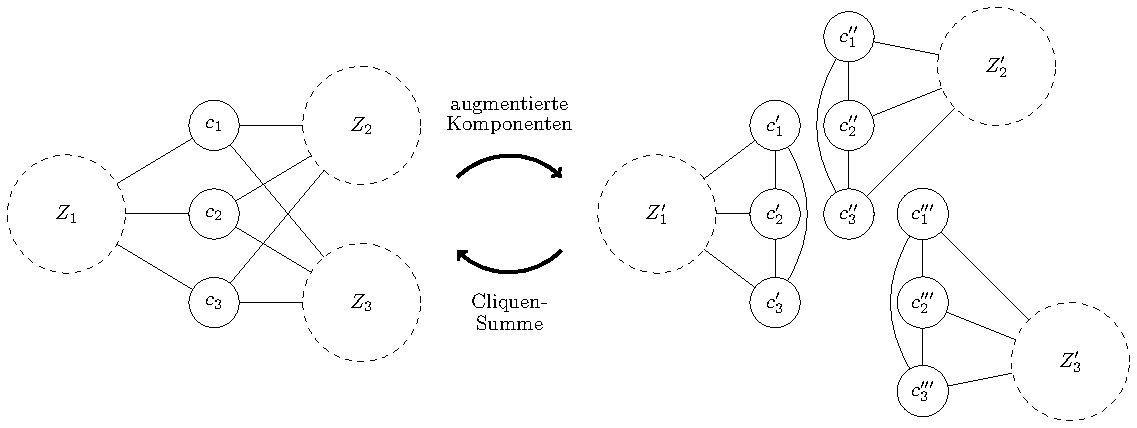
\includegraphics[keepaspectratio]{bilder/Augmentierte_Komponenten.pdf}
  \caption{Der linke Graph wird in drei augmentierte Komponenten durch den \dd-Separator $C = \{c_1, c_2, c_3\}$ geteilt.
           Alle $Z_i$ und $Z_i'$ stellen Teilgraphen dar, die zur Übersicht zu einem Knoten zusammengefügt wurden.
           Die drei rechten Graphen können durch die Cliquen-Summe der Cliquen $\{c_1', c_2', c_3'\}$ sowie $\{c_1'', c_2'', c_3''\}$ und $\{c_1''', c_2''', c_3'''\}$ den rechten Graph erzeugen.
           Während der Cliquen-Summen Operation dürfen die Kanten, die die Knoten in den Cliquen verbinden, gelöscht werden.}
  \label{fig:AugmentierteKomponenten}
\end{figure}

% kapitel3.tex
\chapter{Algorithmus von Kezdy und McGuinness}
\label{cha:algorithmuskezdymcguinness}

Da die Arbeit auf dem sequenziellen Algorithmus von Kezdy und McGuinness, den sie in \cite{Kez92} vorstellen, beruht, wird er im Folgenden erklärt.
Als Eingabe wird ein ungerichteter Graph ohne Mehrfachkanten erwartet, ausgegeben wird, ob ein $K_5$-Minor enthalten ist oder nicht.
Für den Fall, dass einer gefunden wurde, kann zusätzlich ausgegeben werden, welche Knoten den Minor formen.
Die Laufzeit liegt in $\mathcal{O}(n^2)$

Planaritästests können bereits in linearer Laufzeit entscheiden, ob ein Graph planar ist oder einen \kf- \bzw \kdd-Minor enthält.
Es muss lediglich der Fall behandelt werden, in dem der der Test stoppt, weil er einen \kdd-Minor gefunden hat, denn es kann nicht garantiert werden, ob zusätzlich ein \kf-Minor enthalten ist.
Als Lösung testet der Algoritmus von Kezdy und McGuiness, ob ein gefundener \kdd-Minor ein gültiger $3$-Separator ist und zerlegt \ggf den Graph in augmentierte Komponenten.
Anschließend kann der Planaritästest auf die einzelnen Komponenten rekursiv angewendet werden.

Um das zentrale Theorem aus \cite{Kez92}, welches den \kdd-Minor untersucht, zu erklären, wird zunächst die Gültigkeit augmentierter Komponenten behandelt:
\begin{theorem}\label{Theorem33}
  Für $k \geq 3$: Sei $G$ ein $k$-zusammenhängender Graph und $C$ ein $k$-Schnitt in $G$.
  Alle durch $C$ definierten augmentierten Komponenten sind Minoren von $G$, falls es entweder mindestens $k$ Komponenten sind oder mindestens zwei der Komponenten jeweils aus mehr als einem Knoten bestehen.
\end{theorem}
\begin{beweis}
  Seien $c_1, c_2, ..., c_k$ die Knoten von $C$ und $Z = \{Z_1, Z_2, ..., Z_k\}$ \bzw $Z = \{Z_1, Z_2, ..., Z_{k-1}\}$ die Zusammenhangskomponenten, die durch $G \cap C$ entstehen.
  Die zugehörigen augmentierten Komponenten seien $A_1, A_2, ..., A_k$ \bzw $A_1, A_2, ..., A_{k-1}$.
  Betrachtet wird eine beliebige dieser augmentierten Komponenten $A_i$.
  Der Definition der augmentierten Komponenten nach finden sich bereits alle Knoten von $A_i$ in $G$ wieder.
  Weiterhin enthält $G$ mindestens alle Kanten in $A_i \cap C$ sowie die verbindenden Kanten zwischen $A_i$ und $C$.
  Jedoch bilden in $A_i$ die Knoten von $C$ eine Clique, es existieren also \ggf Kanten zwichen den Knoten von $C$ in $A_i$, die es nicht in $G$ gibt
  Es bleibt zu zeigen, dass die Kanten, die für diese Clique in $A_i$ nötig sind, durch Kantenkontraktionen in $G$ erzeugt werden können.
  Dadurch, dass $G$ $k$-zusammenhängend ist, besitzt jede Zusammenhangskomponente von $G \cap C$ Kanten zu $c_1, c_2, ..., c_k$.
  Würde eine Kante zu einem Knoten $c_j$ mit $1 \leq j \leq k$ fehlen, wäre ein $k-1$-Schnitt bestehend aus $C \setminus c_j$ möglich, was im Widerspruch zu dem $k$-Zusammenhang stehen würde.
  Das Theorem unterscheided nun zwei Fälle, um die fehlenden Kanten bereitstellen zu können:
  \begin{enumerate}
    \item Es existieren $k$ Zusammenhangskomponenten.
          Wird $A_i$ betrachtet, kommen die Knoten in $Z \setminus Z_i$ in Frage, um durch Kantenkontraktionen die fehlenden Kanten für die Clique von $C$ in $A_i$ zu erzeugen.
          Um die Kanten von $C$ in $A_i$ in $G$ zu erzeugen, kann zunächst der Pfad, der $c_1$ mit $Z_1$ verbindet, kontrahiert werden.
          Anschließend ist $c_1$ mit allen Knoten in $C$ verbunden.
          Dies kann analog für alle Knoten in $C$ und den entsprechenden Zusammenhangskomponenten durchgeführt werden außer für $c_i$, da $A_i$ der gesuchte Minor ist.
          Allerdings ist $c_i$ aufgrund des $k$-Zusammenhangs mit allen anderen Zusammenhangskomponenten verbunden und nach den beschriebenen Kontraktionen bildet $C$ eine Clique.
    \item Es existieren $k-1$ Komponenten, aber mindestens zwei bestehen aus mehr als einem Knoten.
          Analog zum vorherigen Fall können die Pfade zwischen den Knoten von $C$ und den Zusammenhangskomponenten $A$ kontrahiert werden.
          Es fehlt jedoch ein Pfad, da eine Zusammenhangskomponente weniger vorliegt.
          Es gibt mindestens eine Zusammenhangskomponente aus $Z \setminus Z_i$, die aus zwei oder mehr Knoten besteht.
          Da der Graph $k$-zusammenhängend ist, sind mindestens zwei dieser Knoten mit allen in $C$ verbunden, sodass sie durch Kontraktionen mit zwei unterschiedlichen Knoten aus $C$ genutzt werden könnenm um die gesuchte Clique zu erzeugen.
  \end{enumerate}
\end{beweis}

Als nächstes stellen Kezdy und McGuinness fest, dass im Fall eines $3$-Separators der Graph Komponenten zerlegt werden kann:
\begin{theorem}\label{Theorem34}
  Sei $G$ ein $3$-zusammenhängender Graph mit einem $3$-Schnitt $C$, der den Graph in mindestens $3$ Zusammenhangskomponenten zerlegt.
  $G$ hat einen \kf-Minor, falls eine der durch $C$ definierten augmentierten Komponenten einen \kf-Minor enthält.
\end{theorem}
\begin{beweis}
  Zunächst kann festgestellt werden, dass falls eine der augmentierten Komponenten einen \kf-Minor enthält, dieser laut Theorem \ref{Theorem33} auch ein Minor von $G$ ist.
  Es bleibt zu zeigen, dass sich ein \kf-Minor nicht auf zwei augmentierte Komponenten erstreckt, sondern sich ausschließlich in einer befindet.
  Angenommen es gilt \kf \minor $G$ und zwei der Branch-Sets, die den \kf-Minor bilden, befinden sich jeweils vollständig in unterschiedlichen Zusammenhangskomponenten.
  In diesem Fall wäre $C$ ein $3$-Schnitt in dem gefundenen Minor, was im Widerspruch zu dem $4$-Zusammenhang des \kf steht.
\end{beweis}

Das zentrale Theorem ist darauf zurückzuführen, dass jeder Graph ohne \kf-Minor durch Cliquen-Summen von Teilgraphen, die planar oder isomorph zu $W$ sind, gebildet werden kann.\cite{Wag37}
\begin{theorem}\label{Theorem36}
  Sei $G$ ein $3$-zusammenhängender Graph mit einem \kdd-Homeomorph $S$, dessen Knoten gemäß einer 2-Färbung in $R = \{a, b, c\}$ und $B = \{x, y, z\}$ unterteilt sind.
  Eine der folgenden Bedingungen trifft auf $G$ zu:
  \begin{enumerate}
    \item $G$ enthält einen \kf-Minor.\label{Theorem361}
    \item $G$ ist isomorph zu $W$.\label{Theorem362}
    \item $\{a, b, c\}$ bilden einen $3$-Separator, sodass $\{x, y, z\}$ in separaten Komponenten liegen.\label{Theorem363}
    \item $\{x, y, z\}$ bilden einen $3$-Separator, sodass $\{a, b, c\}$ in separaten Komponenten liegen.\label{Theorem364}
  \end{enumerate}
\end{theorem}
Durch die Theoreme \ref{Theorem33} und \ref{Theorem34} wurde gezeigt, dass der Graph in den Fällen \ref{Theorem363} und \ref{Theorem364} in augmentierte Komponenten zerlegt und darauf der Planaritästest ausgeführt werden kann.
Daher stellen die Autoren einige Lemmata auf, mit denen untersucht wird, ob $S$ einen \kf-Minor enthält - also ob Bedingung \ref{Theorem361} zutrifft.

% TODO: Bilder zum Lemma und M
\begin{lemma}\label{Lemma32}
  Sei $G$ ein $3$-zusammenhängender Graph und $S$ ein \kdd-Homeomorph in $G$.
  Hat ein Knoten $w$ in $G \cap S$ drei Pfade zu Knoten in $S$, die nicht alle im selben Branch-Fan liegen, enthält $G$ einen \kf-Minor.
\end{lemma}
\begin{beweis}
  Seien $t, u, v$ die drei Endpunkte der Pfade in $S$.
  Mindestens einer von ihnen ist ein innerer Knoten, da sonst alle im selben Branch-Fan liegen würden.
  Sei \oBdA $t$ ein solcher innerer Knoten auf dem Pfad $P(a, x)$.
  Folglich können $u$ und $v$ nicht beide in $F(a)$ oder $F(x)$ liegen, sonst lägen alle drei im gleichen Branch-Fan.
  \begin{enumerate}
    \item $u$ und $v$ sind nicht im gleichen Branch-Fan wie $t$. \label{Lemma321}
          Dann müssen $u$ und $v$ ebenfalls innere Knoten sein, im Beispiel auf den Pfaden $P(y, b)$ \bzw $P(z, c)$.
          Es kann ein $M$-Minor durch folgende Kontraktionen erzeugt werden: $u$ mit einem der roten und $v$ mit einem der blauen Knoten (analog $u$ mit blau und $v$ mit rot) sowie $P(w, t)$.
    \item $u$ oder $v$ liegen auf $P(a, x)$. \label{Lemma322}
          Sei \oBdA $u \in P(a, x)$.
          Da $t$ ebenfalls in diesem Pfad liegt, gilt $\{t, u\} \in F(a) \cup F(x)$, sodass $v$ nicht in diesen beiden Branch-Fans liegen kann.
          Es können $t$ und $v$ getauscht werden, sodass eine Reduktion auf Fall \ref{Lemma321} erreicht wird.
    \item Entweder $u$ oder $v$ liegen im gleichen Branch-Fan wie $t$. \label{Lemma323}
          Sei \oBdA $u \in F(x) \cap P(a, x)$, im Beispiel auf dem Pfad $P(b, x)$.
          Es sind $\{t, u\} \in F(x)$, weshalb $v$ in einem anderen Branch Fan sein muss.
          Da alle roten Knoten in $F(x)$ liegen, gilt konkreter $v \in (F(y) \cup F(z)) \cap \{a, b, c\}$
          Es können $P(b, u)$ kontrahiert werden sowie je nach Fall entweder $P(v, y)$ oder $P(v, z)$.
          Wird $P(w, t)$ ebenfalls kontrahiert, entsteht erneut ein $M$-Minor.
  \end{enumerate}
\end{beweis}

% kapitel3.tex
\chapter{Wagner Struktur}
\label{cha:wagnerstruktur}

% kapitel5.tex
\chapter{Implementierung}
\label{cha:implementierung}

% kapitel6.tex
\chapter{Experimentelle Analyse}
\label{cha:analyse}

Die Implementierung des Algorithmus von Kezdy und McGuinness wurde mit dem Planaritätstest von Boyer und Myrvold in OGDF verglichen.
Um den Fehler durch äußere Einflüsse bei geringer Laufzeit zu minimieren, wurde die Zeit von mehreren Iterationen gemessen und anschließend gemittelt.
Einerseits wurden beide Algorithmen auf der \emph{Rome-Library}, einer in \cite{BGLT+97} Testmenge von Graphen, ausgeführt.
Die insgesamt $11528$ Graphen bestehen aus $10$ bis $100$ Knoten.
$8249$ sind nicht planar, davon enthalten $7897$ einen \kf-Minor.

Andererseits wurde ein in \OGDF enthaltener Generator genutzt, um zufällige Graphen mit bis zu $10000$ Knoten und variierender Kantenanzahl zu erzeugen.
Um vor allem den Kern des Kezdy-McGuinness Algorithmus, dem Behandeln von \kdd-Minoren, zu Testen, wurden ausschließlich $3$-zusammenhängende Graphen erzeugt.
Dadurch beeinflussen weder Block-Cut Trees noch SPQR-Bäume die Laufzeit.
Außerdem wird kein Zertifikat für den Fall erstellt, dass ein \kf-Minor gefunden wurde.
Ist kein \kf-Minor im Eingabegraph enthalten, liegt ein Zertifikat vor, da während des Algorithmus die Wagner-Struktur aufgebaut wurde.

Getestet wurde auf einem Intel Core i7-9700k mit 3GHz und 32GB RAM.
Als Compiler wurde der GCC 7.3.0 verwendet.

\begin{figure}[H]
  \centering
  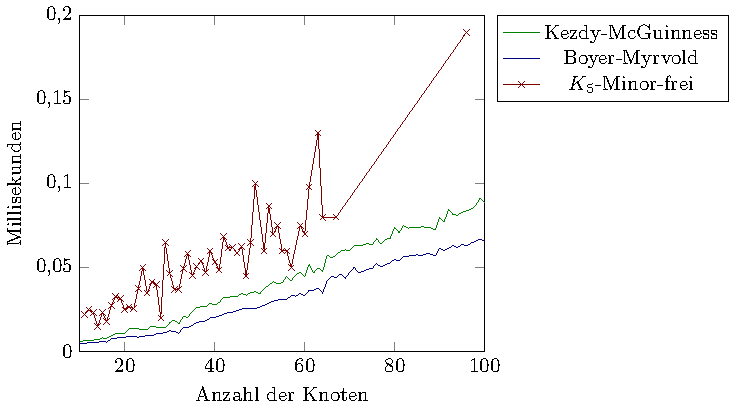
\includegraphics[width=\textwidth,height=\textheight,keepaspectratio]{plots/Benchmarks_Rome.pdf}
  \caption{Benchmark mit den Graphen der Rome Library.}
  \label{fig:Benchmarks-Rome}
\end{figure}

In \Abb \ref{fig:Benchmarks-Rome} ist die Laufzeit in Millisekunden pro Graph zu sehen.
Es fällt auf, dass sich die Laufzeit vom Kezdy-McGuinness-Algorithmus (grün) stark an der des Planaritätstests (blau) orientiert und damit eher linear als quadratisch ist.
Die theoretische Worst-Case-Laufzeit tritt in diesem Anwendungsfall selten auf, da, wie in \Abb \ref{fig:Statistics-Rome} zu sehen, die meisten Graphen entweder planar sind oder einen \kf-Minor enthalten.
Ist ein Graph planar, kann der Algorithmus nach einmaligem Ausführen des Planaritätstests beendet werden, sodass die Laufzeit fast identisch zu der des Planaritätstests ist.
Der Mehraufwand begründet sich in dem Aufbauen der nötigen Datenstrukturen wie der Wagner-Struktur oder einer Kopie des Eingabegraphen, die aus $3$-zusammenhängende Komponenten besteht.
Außerdem findet der Planaritätstest oft direkt einen \kf-Minor oder einen \kdd-Minor, der kein \dd-Separator ist, sodass auch in den beiden Fällen der Kezdy-McGuinness-Algorithmus nach nur einem Rekursionsschritt terminieren kann.
\Abb \ref{fig:Statistics-Rome} ist zu entnehmen, dass viele Graphen entweder einen \kf-Minor enthalten oder planar sind.
Deshalb wurde in \Abb \ref{fig:Benchmarks-Rome} der Kezdy-McGuinness-Algorithmus (rot) zusätzlich nur auf den \kf-Minor-freien Graphen, die nicht planar sind, ausgeführt.
Da nicht für alle Knotenanzahlen solche Graphen vorliegen, wurden gemessenen Werte durch Kreuze markiert.
Hier wird deutlich, dass der Algorithmus deutlich länger läuft, weil der Planaritätstest \dd-Separatoren findet und rekursiv auf die augmentierten Komponenten angewendet wird.
Generell ist in \Abb \ref{fig:Statistics-Rome} aber zu sehen, dass \dd-Separatoren nur in weniger als $10\%$ der Graphen vorkommen.

\begin{figure}[H]
  \centering
  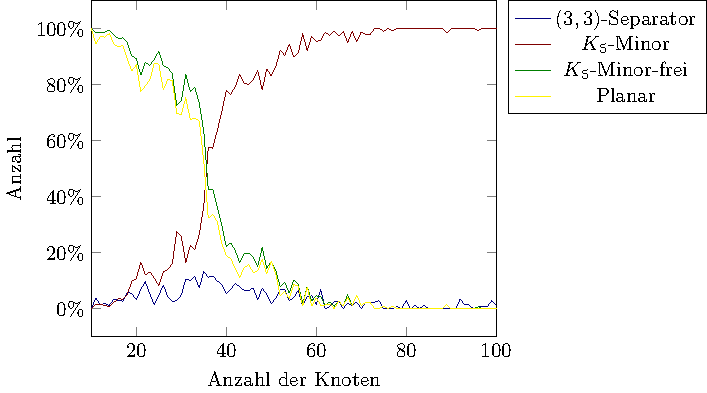
\includegraphics[width=\textwidth,height=\textheight,keepaspectratio]{plots/Statistics_Rome.pdf}
  \caption{Angaben, wie viele Graphen \dd-Separatoren und/oder \kf-Minor enthalten \bzw wie viele planar und/oder \kf-Minor-frei sind.}
  \label{fig:Statistics-Rome}
\end{figure}

\begin{figure}[H]
  \centering
  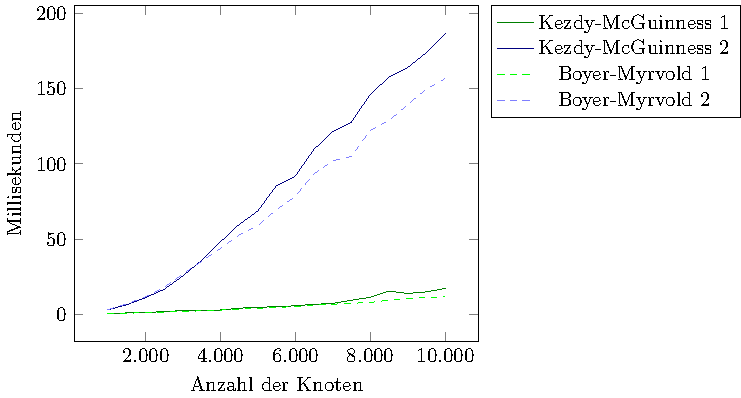
\includegraphics[width=\textwidth,height=\textheight,keepaspectratio]{plots/Benchmarks_Triconnected.pdf}
  \caption{Benchmark $3$-zusammenhängender Graphen mit $n$ Knoten und $2*n$ Kanten (grün) \bzw $10*n$ Kanten.}
  \label{fig:Benchmarks-Triconnected}
\end{figure}

\begin{figure}[H]
  \centering
  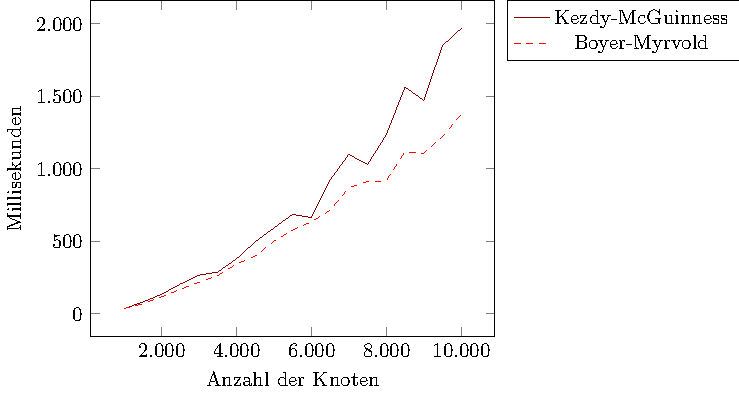
\includegraphics[width=\textwidth,height=\textheight,keepaspectratio]{plots/Benchmarks_TriconnectedVeryDense.pdf}
  \caption{Benchmark $3$-zusammenhängender Graphen mit $n$ Knoten und $f * n$ Kanten für $30 \leq f \leq 100$.}
  \label{fig:Benchmarks-Triconnected-Very-Dense}
\end{figure}

In \Abb \ref{fig:Benchmarks-Triconnected} und \Abb \ref{fig:Benchmarks-Triconnected-Very-Dense} sind die Laufzeiten für größere Graphen zu sehen.
Es wurden für $20$ unterschiedliche Knotengrößen jeweils $25$ Graphen erzeugt und die Messwerte gemittelt.
Die Messungen in \Abb \ref{fig:Benchmarks-Triconnected} decken sich mit den Erkennntnissen, die aus der Rome-Library gewonnen wurden.
Die Graphen in \Abb \ref{fig:Benchmarks-Triconnected-Very-Dense} für größere Kantenanzahlen variieren dagegen deutlicher.
Vermutlich wird für die langsameren Instanzen durch den Planaritätstest ein \kdd-Minor gefunden.
Würde er einen \dd-Separator bilden, müsste die Laufzeit deutlich langsamer sein, wie etwa die Messungen für \kf-Minor-freie Graphen in \Abb \ref{fig:Benchmarks-Rome} zeigen.
Allerdings funktioniert der Test, ob der \kdd-Minor ein \dd-Separator ist, über Tiefensuchen, die durch die deutlich höhere Kantenanzahl länger laufen.
Es sei außerdem erwähnt, dass durch die hohe Kantenanzahl immer ein \kf-Minor enthalten ist.

\ \\

Zuletzt wurden in \Abb \ref{fig:Benchmarks-Small} Graphen mit wenigen Knoten und Kanten getestet.
Es wurden nur $10$ Graphen pro Knotenanzahl erzeugt, dafür jedoch in einem kleineren Intervall.
Dadurch konnte eine stärkere Varianz in der Laufzeit gemessen werden.
In \Abb \ref{fig:Statistics-Small} wurde angegeben, wie viele \dd-Separatoren durchschnittlich gefunden wurden.
Es zeichnet sich ab, dass der Kezdy-McGuinness-Algorithmus schneller ist, umso weniger \dd-Separatoren gefunden werden.
Beispielsweise enthielten von den Graphen mit $700$ Knoten im Schnitt $30\%$ einen \dd-Separator, die Laufzeit lag bei $0,685ms$.
Demgegenüber enthielt keiner der Graphen mit $720$, bis $740$ Knoten einen \dd-Separator, sodass eine schnellere Laufzeit abgelesen werden kann.
Die Laufzeit für Graphen mit $740$ Knoten lag beispielsweise bei nur $0,532ms$ und liefen damit ähnlich schnell, wie die für kleineren Instanzen mit $580$ Knoten.

\begin{figure}[H]
  \centering
  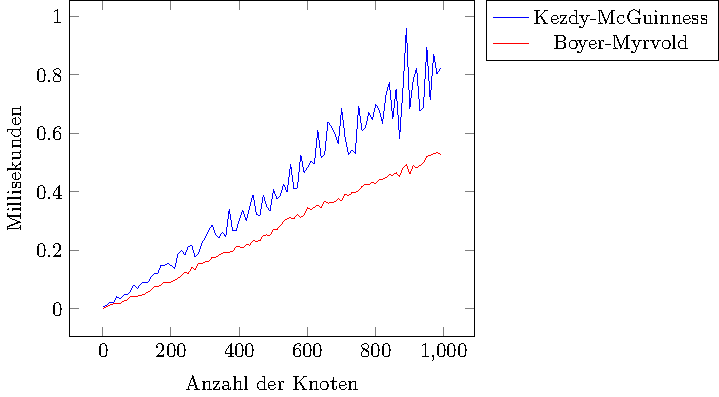
\includegraphics[width=\textwidth,height=\textheight,keepaspectratio]{plots/Benchmarks_Small.pdf}
  \caption{Benchmark für Graphen mit $n$ Knoten und $2*n$ Kanten.}
  \label{fig:Benchmarks-Small}
\end{figure}

\begin{figure}[H]
  \centering
  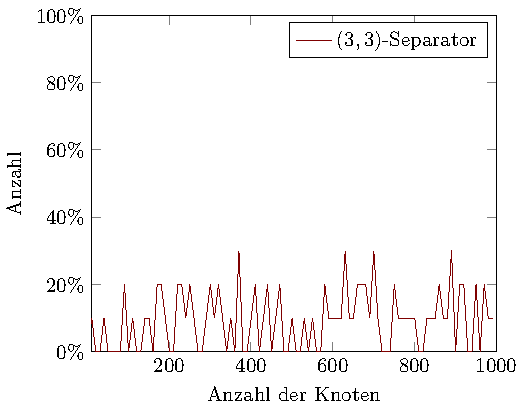
\includegraphics[width=\textwidth,height=\textheight,keepaspectratio]{plots/Statistics_Small.pdf}
  \caption{Angabe, wie viele Graphen mit $n$ Knoten und $2*n$ Kanten einen \dd-Separatoren enthalten.}
  \label{fig:Statistics-Small}
\end{figure}

% fazit.tex
\chapter{Zusammenfassung und Ausblick}
\label{cha:fazit}

Es wurde ein Verfahren vorgestellt, das entscheiden kann, ob ein Graph einen \kf-Minor enthält.
Außerdem wurde erklärt, wie sich \kf-Minor-freie Graphen nach dem Theorem von Wagner aufteilen lassen und eine Baumstruktur gezeigt, die diese Aufteilung widerspiegelt.
Für die Implementierung in OGDF wurden im Wesentlichen Block-Cut Trees und SPQR-Bäume verwendet, um $3$-zusammenhängende Graphen zu erzeugen, und anschließend der Boyer-Myrvold Planaritätstest, um solange \dd-Separatoren zu finden, bis ein \kf-Minor gefunden wurde oder der Graph eindeutig \kf-Minor-frei ist.
Bisher werden Zertifikate für $3$-zusammenhängende Graphen, die \kf-Minor-frei sind, erzeugt.
Vor allem die Berechnung von \kf-Modellen im Eingabegraph kann im Hinblick auf den praktischen Nutzen von wesentlicher Bedeutung sein.
Auch kann es für einige praktische Anwendungen sinnvoll sein, den Algorithmus zu erweitern, sodass mehrere \kf-Minoren in Graphen zu berechnen werden können.
Dafür könnte der Algorithmus \zB so angepasst werden, dass in gefundenen \kf-Minoren einzelne Kanten verändert (kontrahiert, entfernt) werden, um bei einem erneuten Durchlauf einen anderen \kf-Minor zu finden.
So könnten viele \kf-Minoren gefunden werden, die sich allerdings kaum unterscheiden und eine hohe Laufzeit verursachen.
Ein weiterer Ansatz könnte daraus bestehen, den Algorithmus nicht zu terminieren, wenn in einer augmentierten Komponente ein \kf-Minor gefunde wurde.
Wird stattdessen in den übrigen Komponenten weitergesucht, ist es möglich, \kf-Minoren zu finden, die sich stark voneinander unterscheiden.
Tests während der experimentellen Analyse haben jedoch angedeutet, dass auf diese Art meist nur einstellige Mengen von \kf-Minoren in den getesteten Graphen gefunden werden konnten.
Da es sich um ein heuristisches Verfahren handelt, wurde es nicht mit in die Arbeit aufgenommen -- einige praktische Anwendungen, wie die Berechnung des maximalen Schnittes in Graphen, die nicht \kf-Minor-frei sind, könnten jedoch davon profitieren.
Es steht aus, diese beiden Ansätze in einer experimentellen Analyse für solche speziellen Anwendungsfälle zu prüfen.

Darüber hinaus gibt es Ansätze in \cite{Li11}, \cite{ReL08} und \cite{ReL}, die in theoretisch linearer Laufzeit entscheiden, ob ein Graph \kf-Minor-frei ist.
Allerdings bleibt die Frage offen, ob eine Implementierung in der Praxis eine bessere Laufzeit aufweisen würde, da teils mit großen Konstanten gearbeitet wird.

Letztlich wären weitere Laufzeittests speziell für Graphen, die nicht planar sind und keinen \kf-Minor enthalten, interessant, da vor allem dann hohe Laufzeiten in der Praxis auftreten können.
Für alle getesteten Graphen konnte der Algorithmus dagegen in wenigen Sekunden entscheiden, ob ein \kf-Minor in einem Graph enthalten ist.


% Anhang (optional)
\appendix
% anhang.tex
\chapter{Weitere Informationen}


%Abbildungsverzeichnis
\listoffigures
\addcontentsline{toc}{chapter}{Abbildungsverzeichnis}
\cleardoublepage

% Algorithmenverzeichnis
\listofalgorithms
\addcontentsline{toc}{chapter}{Algorithmenverzeichnis}
\cleardoublepage

% Symbolverzeichnis (optional)
\renewcommand{\symheadingname}{Symbolverzeichnis}
\listofsymbols
\addcontentsline{toc}{chapter}{Symbolverzeichnis}
\cleardoublepage

% Literaturverzeichnis
\bibliographystyle{gerplain}
\bibliography{options/literatur}
\addcontentsline{toc}{chapter}{\bibname}

% Erklaerung
\thispagestyle{myheadings}
%\markboth{}{ERKLÄRUNG}
%\addcontentsline{toc}{chapter}{Erklärung}
\markboth{}{EIDESSTATTLICHE VERSICHERUNG}
\addcontentsline{toc}{chapter}{Eidesstattliche Versicherung}
% erklaerung.tex
\parindent 0pt
\cleardoublepage

{\centering \hspace*{1cm}\Large \textbf{Eidesstattliche Versicherung} 

}

\normalsize
\vspace*{1cm}

\parbox{5cm}{ \centering \MeinNachname, \MeinVorame 
\vspace*{0,1cm}
\hrule
\vspace*{0,1cm}
\strut \small \ Name, Vorname} \hfill
\parbox{3cm}{ \centering \MeineMatrikelnummer 
\vspace*{0,15cm}
\hrule
\vspace*{0,1cm}
\strut \small \ Matr.-nr.}

\vspace*{1cm}

Ich versichere hiermit an Eides statt, dass ich die vorliegende \MeineArbeit mit dem Titel

\vspace{0,25cm}
{
\centering
\textbf{\MeinTitel}

}
\vspace{0,25cm}

selbstständig und ohne unzulässige fremde Hilfe erbracht habe. Ich habe keine anderen als die angegebenen Quellen und Hilfsmittel benutzt sowie wörtliche und sinngemäße Zitate kenntlich gemacht. Die Arbeit hat in gleicher oder ähnlicher Form noch keiner Prüfungsbehörde vorgelegen. 
\vspace*{1cm}

\parbox{6.2cm}{ Dortmund, den \today
\vspace*{0,1cm}
\hrule
\vspace*{0,2cm}
\strut \small \ Ort, Datum} \hfill
\parbox{5cm}{ \color{white} Platzhalter \color{black}
\vspace*{0,1cm}
\hrule
\vspace*{0,2cm}
\strut \small \ Unterschrift}

\vspace*{1,5cm}

\textbf{Belehrung:} \vspace{0,25cm}
\newline
Wer vorsätzlich gegen eine die Täuschung über Prüfungsleistungen betreffende Re\-ge\-lung einer Hochschulprüfungsordnung verstößt, handelt ordnungswidrig. Die Ordnungs\-widrig\-keit kann mit einer Geldbuße von bis zu 50.000,00 \euro\ geahndet werden. Zuständige Verwaltungsbehörde für die Verfolgung und Ahndung von Ordnungswidrigkeiten ist der Kanzler/ die Kanzlerin der Technischen Universität Dortmund. Im Falle eines mehrfachen oder sonstigen schwerwiegenden Täuschungsversuches kann der Prüfling zudem exmatrikuliert werden. (\textsection\ 63 Abs. 5 Hochschulgesetz - HG - )
\vspace{0,25cm} \newline
Die Abgabe einer falschen Versicherung an Eides statt wird mit Freiheitsstrafe bis zu 3 Jahren oder mit Geldstrafe bestraft.
\vspace{0,25cm} \newline
Die Technische Universität Dortmund wird gfls. elektronische Vergleichswerkzeuge (wie z.B. die Software „turnitin“) zur Überprüfung von Ordnungswidrigkeiten in Prüfungsverfahren nutzen.
\vspace{0,25cm} \newline
Die oben stehende Belehrung habe ich zur Kenntnis genommen:
\vspace*{1cm}

\parbox{6.2cm}{ Dortmund, den \today
\vspace*{0,1cm}
\hrule
\vspace*{0,1cm}
\strut \small \ Ort, Datum} \hfill
\parbox{5cm}{ \color{white} Platzhalter \color{black}
\vspace*{0,1cm}
\hrule
\vspace*{0,1cm}
\strut \small \ Unterschrift}

%
%\addcontentsline{toc}{chapter}{Eidesstattliche Versicherung}


%\cleardoublepage
%\textbf{
%Die unten stehende Erklärung ist nur für Diplomarbeiten geeignet.
%Für Bachelor- und Masterarbeiten diese Seite vollständig aus der Arbeit entfernen und stattdessen die vorgebene Erklärung vom Prüfungsamt mit in die Arbeit einbinden.
%Diese muss nicht im Inhaltsverzeichnis auftauchen und muss auch keine Seitenzahl haben.
%Einfach nur das ausgefüllte Blatt ganz am Ende mit in die Arbeit einbinden.
%Die Erklärung findet sich auf der Seite des Prüfungsamts (TU Homepage $\rightarrow$ Studierende $\rightarrow$ Prüfungsangelegenheiten) unter dem Punkt Bachelor- und Masterarbeiten.
%Diesen fett gedruckten Text auf jeden Fall aus der Arbeit entfernen!
%}
%\\
%\normalsize
%Hiermit versichere ich, dass ich die vorliegende Arbeit selbstständig verfasst habe und keine anderen als die angegebenen Quellen und Hilfsmittel verwendet sowie Zitate kenntlich gemacht habe.\\\\
%Dortmund, den \today \\\\\\\\
%Muster Mustermann
% EOF
\cleardoublepage

\end{document}
% EOF
